\documentclass{beamer}

% Some common packages
\usepackage{graphicx, color}
\usepackage{alltt}
\usepackage{booktabs, calc, rotating}
\usepackage[round]{natbib}
\usepackage{multicol}
\usepackage{amsmath, amsbsy, amssymb, amsthm, graphicx}
\usepackage[english]{babel}
\usepackage{xkeyval} 
\usepackage{xfrac}
\usepackage[normalem]{ulem}
\usepackage{fancyvrb} 
\usepackage{tikz, geometry, tkz-graph, xcolor}
\usepackage[latin1]{inputenc}
\usepackage{times}
\usepackage[T1]{fontenc}

% Shortcuts
\newcommand{\empr}[1]{{\emph{\color{red}#1}}}
\newcommand{\cov}{\mathrm{cov}}
\newcommand{\pkg}[1]{{\textbf{\texttt{#1}}}}
\newcommand{\dif}{\mathrm{d}}
\newcommand{\bigbrk}{\vspace*{2in}}
\newcommand{\smallbrk}{\vspace*{.1in}}
\newcommand{\midbrk}{\vspace*{1in}}
\newcommand{\red}[1]{{\color{red}#1}}
\newcommand{\blue}[1]{{\color{blue}#1}}
\newcommand{\green}[1]{{\color{green}#1}}
\newcommand{\calc}[1]{{\fbox{\mbox{#1}}}}
\newcommand{\Var}{\mathrm{Var}}%
\newcommand{\Cov}{\mathrm{Cov}}%

\mode<presentation>
{
	\usetheme{UTD}
	\usecolortheme[RGB={200,0,0}]{structure}
	\setbeamercovered{transparent}
}

% fancy for Verbatim?
\fvset{frame=single,framesep=1mm,fontfamily=courier,fontsize=\scriptsize,numbers=left,framerule=.3mm,numbersep=1mm,commandchars=\\\{\}}


\title[Survival Analysis]{Applied Survival Analysis Using R\\ Chapter 8: Time Dependent Covariates}
\author[Qi Guo]{Qi Guo}
\institute[UTD]{Department of Mathematical Sciences \\ 
	The University of Texas at Dallas}
\date{April, 16 2019}
	
\begin{document}

\begin{frame}
  \titlepage
\end{frame}

% Set up UTD backgroud
\setbeamercolor*{item}{fg=red}
\bgroup
\usebackgroundtemplate{
\tikz[overlay,remember picture] \node[opacity=0.05, at=(current page.center)] {
   
\includegraphics[height=\paperheight,width=\paperwidth]{UTDbg}};}


\section[Outline]{}
\begin{frame}
  \tableofcontents
\end{frame}

\section{Introduction}
\begin{frame}
\frametitle{Introduction}
\begin{itemize}
\item The values of the covariates must be determined at time $t=0$, when the patient enters the study, and \empr{remain constant} thereafter.
\item  Such data \empr{evolve over time}, and it would be improper to use the value a covariate to model survival information that is observed before the covariate's value is known.
\item \empr{An intervention that occurs} after the start of the trial, or \empr{a covariate (such as air pollution exposure) that changes} values over the course of the study are two examples of time dependent variables.
\end{itemize}
\end{frame}

\pagebreak
\begin{frame}[fragile]
\frametitle{Example}
\begin{problock}{Transplant Program}
The study of the survival of patients who had been enrolled into the \empr{transplant program} appeared to show that patients who received heart transplants \empr{lived significantly longer} than those who did not.
\end{problock}
\begin{Verbatim}
> result.heart <- coxph(Surv(futime, fustat) ~ transplant + age
 + surgery,data=jasa)
> summary(result.heart)
   n= 103, number of events= 75
            coef       exp(coef)     se(coef)      z      Pr(>|z|)
transplant -1.71711     0.17958      0.27853    -6.165    7.05e-10 ***
age         0.05889     1.06065      0.01505     3.913    9.12e-05 ***    
surgery    -0.41902     0.65769      0.37118    -1.129    0.259 
Signif. codes: 0 *** 0.001 ** 0.01 * 0.05 . 0.1 
\end{Verbatim}
\end{frame}

\pagebreak
\begin{frame}
\frametitle{Problem}
\begin{itemize}
\item The key covariate is ``\texttt{transplant}'', which takes the value 1 for those patients who received a heart transplant and 0 for those who did not.
\item The estimate of the transplant coefficient is -1.717, and the p-value is very small. This result may appear to indicate that transplants are extremely effective in increasing the lifespan of the recipients.
\item The problem here is that receipt of a transplant is a \empr{time dependent covariate}; patients who received a transplant had to live long enough to receive that transplant.
\end{itemize}
\end{frame}

\section{Landmark}
\begin{frame}[fragile]
\frametitle{Fix}
\begin{itemize}
\item Define a ``\texttt{landmark}'' time to \empr{divide} patients into two groups, patients who receive the intervention prior to the landmark go into the intervention group and those who did not are placed in the comparison group.
\item Approach:
\begin{itemize}
\item Only patients who survive up to the landmark are included in the study.
\item All patients remain in their originally assigned group regardless of what happens in the future.
\end{itemize}
\item For the heart transplant data, we may set a landmark at \empr{30 days}.
\end{itemize}
\end{frame}

\pagebreak
\begin{frame}[fragile]
\frametitle{Outcome}
\begin{itemize}
\begin{Verbatim}
> ind30 <- jasa$futime >= 30
> transplant30 <- \{\{jasa$transplant == 1\}\&\{jasa$wait.time < 30\}\}
> summary(coxph(Surv(futime, fustat)~transplant30 + age 
+ surgery, data=jasa, subset=ind30))
  n= 79, number of events= 52
                     coef   exp(coef)  se(coef)    z    Pr(>|z|)
transplant30TRUE  -0.04214  0.95874    0.28377  -0.148  0.8820 
age                0.03720  1.03790    0.01714   2.170  0.0300 *    
surgery           -0.81966  0.44058    0.41297  -1.985  0.0472 *
Signif. codes: 0 *** 0.001 ** 0.01 * 0.05 . 0.1 
\end{Verbatim}
\item Conclusion: The coefficient for transplant30 (a true/false indicator for transplant within the first 30 days) is -0.042, and the p-value is 0.88,there is \empr{little or no difference} in survival between those who got a transplant and those who did not.
\end{itemize}
\end{frame}

\section{Model as a time dependent variable}
\begin{frame}
\frametitle{Modify the partial likelihood function}
\begin{itemize}
\item We have no guidance as to when to set the landmark.
\item Better way is to directly model the variable ``\texttt{transplant}'' as a time dependent variable, but important \empr{adjustments are required to obtain unbiased estimates}.
\item Modify \empr{the partial likelihood function} to accommodate these types of variables
\begin{equation}
L(\beta) = \prod\limits_{i=1}^{D}\frac{\psi_{ii}}{\sum\limits_{k\in R_i}^{}\psi_{ki}}
\end{equation}
where $\psi_{ki} = e^{z_k(t_i)\beta}$, in Chapter 5 we fixed at time 0 so $z_k(t_i)=z_k$ for all failure time $t_i$.
\end{itemize}
\end{frame}

\pagebreak
\begin{frame}
\frametitle{Example}
\begin{figure}
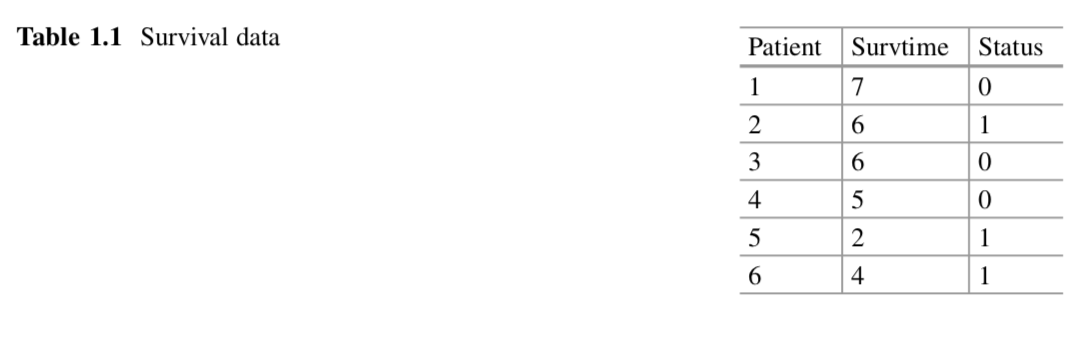
\includegraphics[scale = .3]{001.png}
\end{figure}
\begin{itemize}
\item Patient $\#2$ is the first to fail, at $t=5$. At this time, all six patients are at risk, but only one, Patient $\#95$, has had a transplant at this time, this is denominator, and numerator is 1 due to no-transplant died, so the partial likelihood function:
\end{itemize}
\begin{equation}
L(\beta) = \frac{1}{5+e^{\beta}}\cdot \frac{1}{4+e^{\beta}}\cdot  \frac{e^{\beta}}{2+2e^{\beta}}\cdot \frac{1}{2+e^{\beta}}\cdot \frac{e^{\beta}}{1+e^{\beta}}\cdot \frac{e^{\beta}}{e^{\beta}}
\end{equation}
\end{frame}

\pagebreak
\begin{frame}[fragile]
\frametitle{Transform the data}
\begin{itemize}
\item If it has wait.time, divided into two parts, first 0-wait.time(tstart), second wait.time-futime(tstop)
\begin{Verbatim}
> sdata <- tmerge(heart.simple, heart.simple, id=id, 
death=event(futime, fustat),transpl=tdc(wait.time)) 
> heart.simple.counting <- sdata[,-(2:5)]# drop columns 2 through 5
> heart.simple.counting
  id   tstart   tstop   death   transpl 
1  2     0        5       1        0 
2  5     0       17       1        0 
3  10    0       11       0        0 
4  10   11       57       1        1 
5  12    0        7       1        0 
6  28    0       70       0        0 
7  28   70       71       1        1 
8  95    0        1       0        0 
9  95    1       15       1        1 
\end{Verbatim}
\end{itemize}
\end{frame}

\pagebreak
\begin{frame}[fragile]
\frametitle{Summary}
\begin{figure}
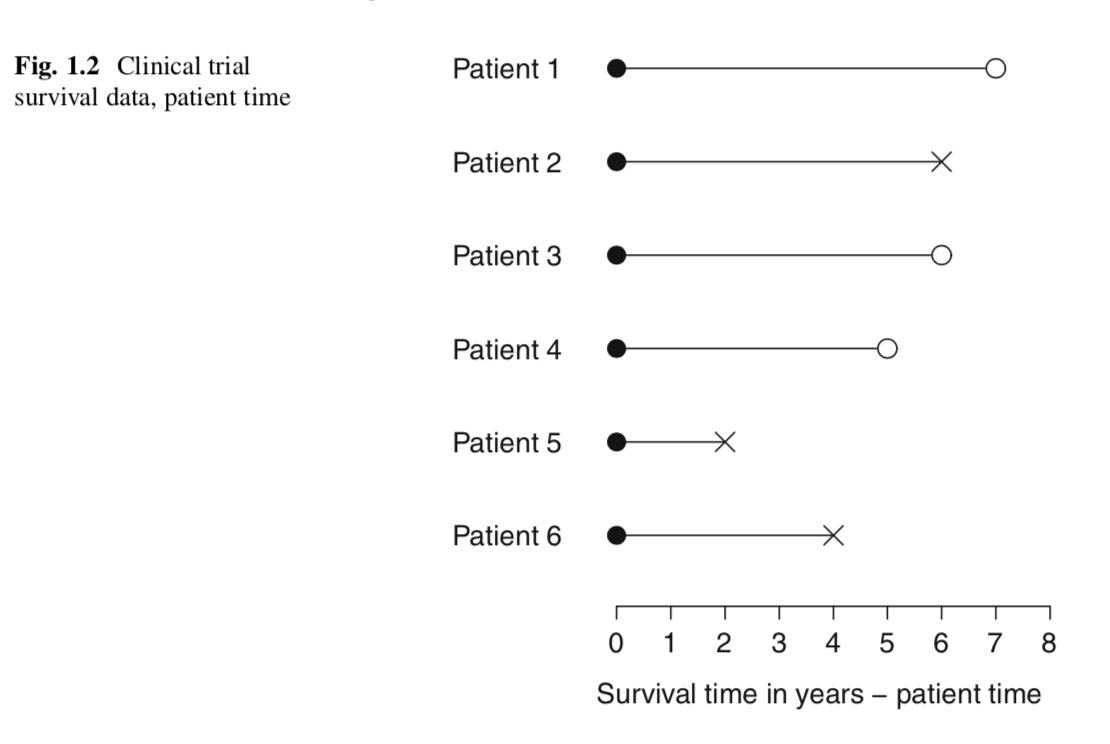
\includegraphics[scale = .3]{002.png}
\end{figure}
\begin{itemize}
\item Use the \texttt{coxph} function as we did with \empr{left-truncated} data:
\begin{Verbatim}
> summary(coxph(Surv(tstart, tstop, death) ~ transpl, 
data=heart.simple.counting))
  n= 9, number of events= 6
         coef   exp(coef)   se(coef)    z   Pr(>|z|) 
transpl 0.2846   1.3292      0.9609   0.296  0.767
\end{Verbatim}
\end{itemize}
\end{frame}

\pagebreak
\begin{frame}[fragile]
\frametitle{Application}
\begin{itemize}
\item Define ``\texttt{tdata}'' as a temporary data set, leaving off the dates and transplant-specific covariates. Also, we add 0.5 to the death time on day 0, and break a tied transplant time.
\begin{Verbatim}
> tdata <- jasa[, -c(1:4, 11:14)]) 
> tdata$futime <- pmax(.5, tdata$futime)
> indx <- \{\{tdata$wait.time == tdata$futime\} \&
!is.na(tdata$wait.time)\}
> tdata$wait.time[indx] <- tdata$wait.time[indx] - .5
> id <- 1:nrow(tdata)
> tdata$id <- id
> sdata <- tmerge(tdata, tdata, id=id, 
death = event(futime, fustat),trans= tdc(wait,time))
> jasa.counting <- sdata[,c(7:11, 2:3)]
> head(jasa.counting)
  id   tstart   tstop   death   trans   suregery       age 
1  1     0        49       1       0        0        30.84463 
2  2     0         5       1       0        0        51.83573 
3  3     0        15       1       1        0        54.29706 
4  4     0        35       0       0        0        40.26283 
5  4    35        38       1       1        0        40.26283
6  5     0        17       1       0        0        20.78576 
\end{Verbatim}
\end{itemize}
\end{frame}

\pagebreak
\begin{frame}[fragile]
\frametitle{Final Conclusion}
\begin{itemize}
\begin{Verbatim}
> summary(coxph(Surv(tstart, tstop, death) ~ trans + surgery +
age, data=jasa.counting))
   n= 170, number of events= 75
             coef      exp(coef)     se(coef)      z      Pr(>|z|)
trans      0.01405      1.01415      0.30822     0.046     0.9636
surgery   -0.77326      0.46150      0.35966    -2.150     0.0316 * 
age        0.03055      1.03103      0.01389     2.199     0.0279 * 
---
Signif. codes: 0 *** 0.001 ** 0.01 * 0.05 . 0.1 
\end{Verbatim}
\item Conclusion: As with the landmark analysis given earlier, that there is no evidence that receiving a heart transplant increases survival. 
\item This method is valid even though (unlike with the landmark method) no data are discarded. 
\end{itemize}
\end{frame}

\section{Predictable Time Dependent Variables}
\begin{frame}[fragile]
\frametitle{Recall}
\begin{itemize}
\item Consider again the pancreatic data in Chapter 4,define a numerical (0/1) group variable, and fit the following model using the ``\texttt{pancreatic2}'' data in the ``\texttt{asaur}'' package:
\begin{Verbatim}
> stage.n <- rep(0, nrow(pancreatic2))
> stage.n[pancreatic2$stage == "M"] <- 1
> result.panc <- coxph(Surv(pfs) ~ stage.n) 
> result.panc
           coef   exp(coef)  se(coef)   z     p 
stage.n   0.593     1.81      0.401   1.48   0.14

Likelihood ratio test=2.43 on 1 df, p=0.119
\end{Verbatim}
\item It shows little evidence of a group difference, and we have a plot of \empr{Schoenfeld residuals} indicated that the hazard ratio appears not to be constant.
\end{itemize}
\end{frame}

\pagebreak
\begin{frame}[fragile]
\frametitle{Using the Time Transfer Function}
\begin{itemize}
\item One way of dealing with this was to use \empr{the Prentice modification} of \texttt{the Wilcoxon test} (using ``\texttt{rho = 1}'' in the ``\texttt{survdiff}'' function)
\item An alternative is to accommodate the changing hazard ratio by defining a time dependent covariate:
\begin{equation}
g(t) = z\cdot \log(t)
\end{equation}
\item Other time dependent function may not work, and the ``\texttt{time transfer}'' function ``\texttt{tt}'' can do this.
\begin{Verbatim}
> result.panc2.tt <- coxph(Surv(pfs) ~ stage.n + tt(stage.n),
tt=function(x,t, ...) x*log(t))
> result.panc2.tt
               coef    exp(coef)    se(coef)   z     p 
stage.n        6.01     407.339      3.060   1.96   0.050
tt(stage.n)   -1.09      0.338       0.589  -1.84   0.065

Likelihood ratio test=6.33 on 2 df, p=0.0423
\end{Verbatim}
\end{itemize}
\end{frame}

\pagebreak
\begin{frame}
\frametitle{Short introduction}
\begin{itemize}
\item We know that the age of a patient increases in lock step with time itself, so can't we treat increasing age as a time dependent variable? The answer is \empr{yes}, but doing so has no effect on the model.
\end{itemize}
\end{frame}



\end{document}